\documentclass{article}
\usepackage{graphicx} % Required for inserting images
\usepackage{indentfirst}
\usepackage[a4paper, margin=3cm]{geometry}
\usepackage{amssymb}
\usepackage[portuguese]{babel}
\usepackage{amsmath}
\usepackage{nicematrix}
\usepackage[breakable]{tcolorbox}
\usepackage{hyperref}
    % Basic figure setup, for now with no caption control since it's done
    % automatically by Pandoc (which extracts ![](path) syntax from Markdown).
    \usepackage{graphicx}
    % Maintain compatibility with old templates. Remove in nbconvert 6.0
    \let\Oldincludegraphics\includegraphics
    % Ensure that by default, figures have no caption (until we provide a
    % proper Figure object with a Caption API and a way to capture that
    % in the conversion process - todo).
    % \usepackage{caption}
    % \DeclareCaptionFormat{nocaption}{}
    % \captionsetup{format=nocaption,aboveskip=0pt,belowskip=0pt}

    \usepackage{float}
    \floatplacement{figure}{H} % forces figures to be placed at the correct location
    \usepackage{xcolor} % Allow colors to be defined
    \usepackage{enumerate} % Needed for markdown enumerations to work
    \usepackage{geometry} % Used to adjust the document margins
    \usepackage{amsmath} % Equations
    \usepackage{amssymb} % Equations
    \usepackage{textcomp} % defines textquotesingle
    % Hack from http://tex.stackexchange.com/a/47451/13684:
    \AtBeginDocument{%
        \def\PYZsq{\textquotesingle}% Upright quotes in Pygmentized code
    }
    \usepackage{upquote} % Upright quotes for verbatim code
    \usepackage{eurosym} % defines \euro

    \usepackage{iftex}
    \ifPDFTeX
        \usepackage[T1]{fontenc}
        \IfFileExists{alphabeta.sty}{
              \usepackage{alphabeta}
          }{
              \usepackage[mathletters]{ucs}
              \usepackage[utf8x]{inputenc}
          }
    \else
        \usepackage{fontspec}
        \usepackage{unicode-math}
    \fi

    \usepackage{fancyvrb} % verbatim replacement that allows latex
    \usepackage{grffile} % extends the file name processing of package graphics
                         % to support a larger range
    \makeatletter % fix for old versions of grffile with XeLaTeX
    \@ifpackagelater{grffile}{2019/11/01}
    {
      % Do nothing on new versions
    }
    {
      \def\Gread@@xetex#1{%
        \IfFileExists{"\Gin@base".bb}%
        {\Gread@eps{\Gin@base.bb}}%
        {\Gread@@xetex@aux#1}%
      }
    }
    \makeatother
    \usepackage[Export]{adjustbox} % Used to constrain images to a maximum size
    \adjustboxset{max size={0.9\linewidth}{0.9\paperheight}}

    % The hyperref package gives us a pdf with properly built
    % internal navigation ('pdf bookmarks' for the table of contents,
    % internal cross-reference links, web links for URLs, etc.)
    \usepackage{hyperref}
    % The default LaTeX title has an obnoxious amount of whitespace. By default,
    % titling removes some of it. It also provides customization options.
    \usepackage{titling}
    \usepackage{longtable} % longtable support required by pandoc >1.10
    \usepackage{booktabs}  % table support for pandoc > 1.12.2
    \usepackage{array}     % table support for pandoc >= 2.11.3
    \usepackage{calc}      % table minipage width calculation for pandoc >= 2.11.1
    \usepackage[inline]{enumitem} % IRkernel/repr support (it uses the enumerate* environment)
    \usepackage[normalem]{ulem} % ulem is needed to support strikethroughs (\sout)
                                % normalem makes italics be italics, not underlines
    \usepackage{mathrsfs}
    

    
    % Colors for the hyperref package
    \definecolor{urlcolor}{rgb}{0,.145,.698}
    \definecolor{linkcolor}{rgb}{.71,0.21,0.01}
    \definecolor{citecolor}{rgb}{.12,.54,.11}

    % ANSI colors
    \definecolor{ansi-black}{HTML}{3E424D}
    \definecolor{ansi-black-intense}{HTML}{282C36}
    \definecolor{ansi-red}{HTML}{E75C58}
    \definecolor{ansi-red-intense}{HTML}{B22B31}
    \definecolor{ansi-green}{HTML}{00A250}
    \definecolor{ansi-green-intense}{HTML}{007427}
    \definecolor{ansi-yellow}{HTML}{DDB62B}
    \definecolor{ansi-yellow-intense}{HTML}{B27D12}
    \definecolor{ansi-blue}{HTML}{208FFB}
    \definecolor{ansi-blue-intense}{HTML}{0065CA}
    \definecolor{ansi-magenta}{HTML}{D160C4}
    \definecolor{ansi-magenta-intense}{HTML}{A03196}
    \definecolor{ansi-cyan}{HTML}{60C6C8}
    \definecolor{ansi-cyan-intense}{HTML}{258F8F}
    \definecolor{ansi-white}{HTML}{C5C1B4}
    \definecolor{ansi-white-intense}{HTML}{A1A6B2}
    \definecolor{ansi-default-inverse-fg}{HTML}{FFFFFF}
    \definecolor{ansi-default-inverse-bg}{HTML}{000000}

    % common color for the border for error outputs.
    \definecolor{outerrorbackground}{HTML}{FFDFDF}

    % commands and environments needed by pandoc snippets
    % extracted from the output of `pandoc -s`
    \providecommand{\tightlist}{%
      \setlength{\itemsep}{0pt}\setlength{\parskip}{0pt}}
    \DefineVerbatimEnvironment{Highlighting}{Verbatim}{commandchars=\\\{\}}
    % Add ',fontsize=\small' for more characters per line
    \newenvironment{Shaded}{}{}
    \newcommand{\KeywordTok}[1]{\textcolor[rgb]{0.00,0.44,0.13}{\textbf{{#1}}}}
    \newcommand{\DataTypeTok}[1]{\textcolor[rgb]{0.56,0.13,0.00}{{#1}}}
    \newcommand{\DecValTok}[1]{\textcolor[rgb]{0.25,0.63,0.44}{{#1}}}
    \newcommand{\BaseNTok}[1]{\textcolor[rgb]{0.25,0.63,0.44}{{#1}}}
    \newcommand{\FloatTok}[1]{\textcolor[rgb]{0.25,0.63,0.44}{{#1}}}
    \newcommand{\CharTok}[1]{\textcolor[rgb]{0.25,0.44,0.63}{{#1}}}
    \newcommand{\StringTok}[1]{\textcolor[rgb]{0.25,0.44,0.63}{{#1}}}
    \newcommand{\CommentTok}[1]{\textcolor[rgb]{0.38,0.63,0.69}{\textit{{#1}}}}
    \newcommand{\OtherTok}[1]{\textcolor[rgb]{0.00,0.44,0.13}{{#1}}}
    \newcommand{\AlertTok}[1]{\textcolor[rgb]{1.00,0.00,0.00}{\textbf{{#1}}}}
    \newcommand{\FunctionTok}[1]{\textcolor[rgb]{0.02,0.16,0.49}{{#1}}}
    \newcommand{\RegionMarkerTok}[1]{{#1}}
    \newcommand{\ErrorTok}[1]{\textcolor[rgb]{1.00,0.00,0.00}{\textbf{{#1}}}}
    \newcommand{\NormalTok}[1]{{#1}}

    % Additional commands for more recent versions of Pandoc
    \newcommand{\ConstantTok}[1]{\textcolor[rgb]{0.53,0.00,0.00}{{#1}}}
    \newcommand{\SpecialCharTok}[1]{\textcolor[rgb]{0.25,0.44,0.63}{{#1}}}
    \newcommand{\VerbatimStringTok}[1]{\textcolor[rgb]{0.25,0.44,0.63}{{#1}}}
    \newcommand{\SpecialStringTok}[1]{\textcolor[rgb]{0.73,0.40,0.53}{{#1}}}
    \newcommand{\ImportTok}[1]{{#1}}
    \newcommand{\DocumentationTok}[1]{\textcolor[rgb]{0.73,0.13,0.13}{\textit{{#1}}}}
    \newcommand{\AnnotationTok}[1]{\textcolor[rgb]{0.38,0.63,0.69}{\textbf{\textit{{#1}}}}}
    \newcommand{\CommentVarTok}[1]{\textcolor[rgb]{0.38,0.63,0.69}{\textbf{\textit{{#1}}}}}
    \newcommand{\VariableTok}[1]{\textcolor[rgb]{0.10,0.09,0.49}{{#1}}}
    \newcommand{\ControlFlowTok}[1]{\textcolor[rgb]{0.00,0.44,0.13}{\textbf{{#1}}}}
    \newcommand{\OperatorTok}[1]{\textcolor[rgb]{0.40,0.40,0.40}{{#1}}}
    \newcommand{\BuiltInTok}[1]{{#1}}
    \newcommand{\ExtensionTok}[1]{{#1}}
    \newcommand{\PreprocessorTok}[1]{\textcolor[rgb]{0.74,0.48,0.00}{{#1}}}
    \newcommand{\AttributeTok}[1]{\textcolor[rgb]{0.49,0.56,0.16}{{#1}}}
    \newcommand{\InformationTok}[1]{\textcolor[rgb]{0.38,0.63,0.69}{\textbf{\textit{{#1}}}}}
    \newcommand{\WarningTok}[1]{\textcolor[rgb]{0.38,0.63,0.69}{\textbf{\textit{{#1}}}}}


    % Define a nice break command that doesn't care if a line doesn't already
    % exist.
    \def\br{\hspace*{\fill} \\* }
    % Math Jax compatibility definitions
    \def\gt{>}
    \def\lt{<}
    \let\Oldtex\TeX
    \let\Oldlatex\LaTeX
    \renewcommand{\TeX}{\textrm{\Oldtex}}
    \renewcommand{\LaTeX}{\textrm{\Oldlatex}}
    % Document parameters
    % Document title
    \title{eigenswift}
    
    
    
    
    
    
    
% Pygments definitions
\makeatletter
\def\PY@reset{\let\PY@it=\relax \let\PY@bf=\relax%
    \let\PY@ul=\relax \let\PY@tc=\relax%
    \let\PY@bc=\relax \let\PY@ff=\relax}
\def\PY@tok#1{\csname PY@tok@#1\endcsname}
\def\PY@toks#1+{\ifx\relax#1\empty\else%
    \PY@tok{#1}\expandafter\PY@toks\fi}
\def\PY@do#1{\PY@bc{\PY@tc{\PY@ul{%
    \PY@it{\PY@bf{\PY@ff{#1}}}}}}}
\def\PY#1#2{\PY@reset\PY@toks#1+\relax+\PY@do{#2}}

\@namedef{PY@tok@w}{\def\PY@tc##1{\textcolor[rgb]{0.73,0.73,0.73}{##1}}}
\@namedef{PY@tok@c}{\let\PY@it=\textit\def\PY@tc##1{\textcolor[rgb]{0.24,0.48,0.48}{##1}}}
\@namedef{PY@tok@cp}{\def\PY@tc##1{\textcolor[rgb]{0.61,0.40,0.00}{##1}}}
\@namedef{PY@tok@k}{\let\PY@bf=\textbf\def\PY@tc##1{\textcolor[rgb]{0.00,0.50,0.00}{##1}}}
\@namedef{PY@tok@kp}{\def\PY@tc##1{\textcolor[rgb]{0.00,0.50,0.00}{##1}}}
\@namedef{PY@tok@kt}{\def\PY@tc##1{\textcolor[rgb]{0.69,0.00,0.25}{##1}}}
\@namedef{PY@tok@o}{\def\PY@tc##1{\textcolor[rgb]{0.40,0.40,0.40}{##1}}}
\@namedef{PY@tok@ow}{\let\PY@bf=\textbf\def\PY@tc##1{\textcolor[rgb]{0.67,0.13,1.00}{##1}}}
\@namedef{PY@tok@nb}{\def\PY@tc##1{\textcolor[rgb]{0.00,0.50,0.00}{##1}}}
\@namedef{PY@tok@nf}{\def\PY@tc##1{\textcolor[rgb]{0.00,0.00,1.00}{##1}}}
\@namedef{PY@tok@nc}{\let\PY@bf=\textbf\def\PY@tc##1{\textcolor[rgb]{0.00,0.00,1.00}{##1}}}
\@namedef{PY@tok@nn}{\let\PY@bf=\textbf\def\PY@tc##1{\textcolor[rgb]{0.00,0.00,1.00}{##1}}}
\@namedef{PY@tok@ne}{\let\PY@bf=\textbf\def\PY@tc##1{\textcolor[rgb]{0.80,0.25,0.22}{##1}}}
\@namedef{PY@tok@nv}{\def\PY@tc##1{\textcolor[rgb]{0.10,0.09,0.49}{##1}}}
\@namedef{PY@tok@no}{\def\PY@tc##1{\textcolor[rgb]{0.53,0.00,0.00}{##1}}}
\@namedef{PY@tok@nl}{\def\PY@tc##1{\textcolor[rgb]{0.46,0.46,0.00}{##1}}}
\@namedef{PY@tok@ni}{\let\PY@bf=\textbf\def\PY@tc##1{\textcolor[rgb]{0.44,0.44,0.44}{##1}}}
\@namedef{PY@tok@na}{\def\PY@tc##1{\textcolor[rgb]{0.41,0.47,0.13}{##1}}}
\@namedef{PY@tok@nt}{\let\PY@bf=\textbf\def\PY@tc##1{\textcolor[rgb]{0.00,0.50,0.00}{##1}}}
\@namedef{PY@tok@nd}{\def\PY@tc##1{\textcolor[rgb]{0.67,0.13,1.00}{##1}}}
\@namedef{PY@tok@s}{\def\PY@tc##1{\textcolor[rgb]{0.73,0.13,0.13}{##1}}}
\@namedef{PY@tok@sd}{\let\PY@it=\textit\def\PY@tc##1{\textcolor[rgb]{0.73,0.13,0.13}{##1}}}
\@namedef{PY@tok@si}{\let\PY@bf=\textbf\def\PY@tc##1{\textcolor[rgb]{0.64,0.35,0.47}{##1}}}
\@namedef{PY@tok@se}{\let\PY@bf=\textbf\def\PY@tc##1{\textcolor[rgb]{0.67,0.36,0.12}{##1}}}
\@namedef{PY@tok@sr}{\def\PY@tc##1{\textcolor[rgb]{0.64,0.35,0.47}{##1}}}
\@namedef{PY@tok@ss}{\def\PY@tc##1{\textcolor[rgb]{0.10,0.09,0.49}{##1}}}
\@namedef{PY@tok@sx}{\def\PY@tc##1{\textcolor[rgb]{0.00,0.50,0.00}{##1}}}
\@namedef{PY@tok@m}{\def\PY@tc##1{\textcolor[rgb]{0.40,0.40,0.40}{##1}}}
\@namedef{PY@tok@gh}{\let\PY@bf=\textbf\def\PY@tc##1{\textcolor[rgb]{0.00,0.00,0.50}{##1}}}
\@namedef{PY@tok@gu}{\let\PY@bf=\textbf\def\PY@tc##1{\textcolor[rgb]{0.50,0.00,0.50}{##1}}}
\@namedef{PY@tok@gd}{\def\PY@tc##1{\textcolor[rgb]{0.63,0.00,0.00}{##1}}}
\@namedef{PY@tok@gi}{\def\PY@tc##1{\textcolor[rgb]{0.00,0.52,0.00}{##1}}}
\@namedef{PY@tok@gr}{\def\PY@tc##1{\textcolor[rgb]{0.89,0.00,0.00}{##1}}}
\@namedef{PY@tok@ge}{\let\PY@it=\textit}
\@namedef{PY@tok@gs}{\let\PY@bf=\textbf}
\@namedef{PY@tok@gp}{\let\PY@bf=\textbf\def\PY@tc##1{\textcolor[rgb]{0.00,0.00,0.50}{##1}}}
\@namedef{PY@tok@go}{\def\PY@tc##1{\textcolor[rgb]{0.44,0.44,0.44}{##1}}}
\@namedef{PY@tok@gt}{\def\PY@tc##1{\textcolor[rgb]{0.00,0.27,0.87}{##1}}}
\@namedef{PY@tok@err}{\def\PY@bc##1{{\setlength{\fboxsep}{\string -\fboxrule}\fcolorbox[rgb]{1.00,0.00,0.00}{1,1,1}{\strut ##1}}}}
\@namedef{PY@tok@kc}{\let\PY@bf=\textbf\def\PY@tc##1{\textcolor[rgb]{0.00,0.50,0.00}{##1}}}
\@namedef{PY@tok@kd}{\let\PY@bf=\textbf\def\PY@tc##1{\textcolor[rgb]{0.00,0.50,0.00}{##1}}}
\@namedef{PY@tok@kn}{\let\PY@bf=\textbf\def\PY@tc##1{\textcolor[rgb]{0.00,0.50,0.00}{##1}}}
\@namedef{PY@tok@kr}{\let\PY@bf=\textbf\def\PY@tc##1{\textcolor[rgb]{0.00,0.50,0.00}{##1}}}
\@namedef{PY@tok@bp}{\def\PY@tc##1{\textcolor[rgb]{0.00,0.50,0.00}{##1}}}
\@namedef{PY@tok@fm}{\def\PY@tc##1{\textcolor[rgb]{0.00,0.00,1.00}{##1}}}
\@namedef{PY@tok@vc}{\def\PY@tc##1{\textcolor[rgb]{0.10,0.09,0.49}{##1}}}
\@namedef{PY@tok@vg}{\def\PY@tc##1{\textcolor[rgb]{0.10,0.09,0.49}{##1}}}
\@namedef{PY@tok@vi}{\def\PY@tc##1{\textcolor[rgb]{0.10,0.09,0.49}{##1}}}
\@namedef{PY@tok@vm}{\def\PY@tc##1{\textcolor[rgb]{0.10,0.09,0.49}{##1}}}
\@namedef{PY@tok@sa}{\def\PY@tc##1{\textcolor[rgb]{0.73,0.13,0.13}{##1}}}
\@namedef{PY@tok@sb}{\def\PY@tc##1{\textcolor[rgb]{0.73,0.13,0.13}{##1}}}
\@namedef{PY@tok@sc}{\def\PY@tc##1{\textcolor[rgb]{0.73,0.13,0.13}{##1}}}
\@namedef{PY@tok@dl}{\def\PY@tc##1{\textcolor[rgb]{0.73,0.13,0.13}{##1}}}
\@namedef{PY@tok@s2}{\def\PY@tc##1{\textcolor[rgb]{0.73,0.13,0.13}{##1}}}
\@namedef{PY@tok@sh}{\def\PY@tc##1{\textcolor[rgb]{0.73,0.13,0.13}{##1}}}
\@namedef{PY@tok@s1}{\def\PY@tc##1{\textcolor[rgb]{0.73,0.13,0.13}{##1}}}
\@namedef{PY@tok@mb}{\def\PY@tc##1{\textcolor[rgb]{0.40,0.40,0.40}{##1}}}
\@namedef{PY@tok@mf}{\def\PY@tc##1{\textcolor[rgb]{0.40,0.40,0.40}{##1}}}
\@namedef{PY@tok@mh}{\def\PY@tc##1{\textcolor[rgb]{0.40,0.40,0.40}{##1}}}
\@namedef{PY@tok@mi}{\def\PY@tc##1{\textcolor[rgb]{0.40,0.40,0.40}{##1}}}
\@namedef{PY@tok@il}{\def\PY@tc##1{\textcolor[rgb]{0.40,0.40,0.40}{##1}}}
\@namedef{PY@tok@mo}{\def\PY@tc##1{\textcolor[rgb]{0.40,0.40,0.40}{##1}}}
\@namedef{PY@tok@ch}{\let\PY@it=\textit\def\PY@tc##1{\textcolor[rgb]{0.24,0.48,0.48}{##1}}}
\@namedef{PY@tok@cm}{\let\PY@it=\textit\def\PY@tc##1{\textcolor[rgb]{0.24,0.48,0.48}{##1}}}
\@namedef{PY@tok@cpf}{\let\PY@it=\textit\def\PY@tc##1{\textcolor[rgb]{0.24,0.48,0.48}{##1}}}
\@namedef{PY@tok@c1}{\let\PY@it=\textit\def\PY@tc##1{\textcolor[rgb]{0.24,0.48,0.48}{##1}}}
\@namedef{PY@tok@cs}{\let\PY@it=\textit\def\PY@tc##1{\textcolor[rgb]{0.24,0.48,0.48}{##1}}}

\def\PYZbs{\char`\\}
\def\PYZus{\char`\_}
\def\PYZob{\char`\{}
\def\PYZcb{\char`\}}
\def\PYZca{\char`\^}
\def\PYZam{\char`\&}
\def\PYZlt{\char`\<}
\def\PYZgt{\char`\>}
\def\PYZsh{\char`\#}
\def\PYZpc{\char`\%}
\def\PYZdl{\char`\$}
\def\PYZhy{\char`\-}
\def\PYZsq{\char`\'}
\def\PYZdq{\char`\"}
\def\PYZti{\char`\~}
% for compatibility with earlier versions
\def\PYZat{@}
\def\PYZlb{[}
\def\PYZrb{]}
\makeatother


    % For linebreaks inside Verbatim environment from package fancyvrb.
    \makeatletter
        \newbox\Wrappedcontinuationbox
        \newbox\Wrappedvisiblespacebox
        \newcommand*\Wrappedvisiblespace {\textcolor{red}{\textvisiblespace}}
        \newcommand*\Wrappedcontinuationsymbol {\textcolor{red}{\llap{\tiny$\m@th\hookrightarrow$}}}
        \newcommand*\Wrappedcontinuationindent {3ex }
        \newcommand*\Wrappedafterbreak {\kern\Wrappedcontinuationindent\copy\Wrappedcontinuationbox}
        % Take advantage of the already applied Pygments mark-up to insert
        % potential linebreaks for TeX processing.
        %        {, <, #, %, $, ' and ": go to next line.
        %        _, }, ^, &, >, - and ~: stay at end of broken line.
        % Use of \textquotesingle for straight quote.
        \newcommand*\Wrappedbreaksatspecials {%
            \def\PYGZus{\discretionary{\char`\_}{\Wrappedafterbreak}{\char`\_}}%
            \def\PYGZob{\discretionary{}{\Wrappedafterbreak\char`\{}{\char`\{}}%
            \def\PYGZcb{\discretionary{\char`\}}{\Wrappedafterbreak}{\char`\}}}%
            \def\PYGZca{\discretionary{\char`\^}{\Wrappedafterbreak}{\char`\^}}%
            \def\PYGZam{\discretionary{\char`\&}{\Wrappedafterbreak}{\char`\&}}%
            \def\PYGZlt{\discretionary{}{\Wrappedafterbreak\char`\<}{\char`\<}}%
            \def\PYGZgt{\discretionary{\char`\>}{\Wrappedafterbreak}{\char`\>}}%
            \def\PYGZsh{\discretionary{}{\Wrappedafterbreak\char`\#}{\char`\#}}%
            \def\PYGZpc{\discretionary{}{\Wrappedafterbreak\char`\%}{\char`\%}}%
            \def\PYGZdl{\discretionary{}{\Wrappedafterbreak\char`\$}{\char`\$}}%
            \def\PYGZhy{\discretionary{\char`\-}{\Wrappedafterbreak}{\char`\-}}%
            \def\PYGZsq{\discretionary{}{\Wrappedafterbreak\textquotesingle}{\textquotesingle}}%
            \def\PYGZdq{\discretionary{}{\Wrappedafterbreak\char`\"}{\char`\"}}%
            \def\PYGZti{\discretionary{\char`\~}{\Wrappedafterbreak}{\char`\~}}%
        }
        % Some characters . , ; ? ! / are not pygmentized.
        % This macro makes them "active" and they will insert potential linebreaks
        \newcommand*\Wrappedbreaksatpunct {%
            \lccode`\~`\.\lowercase{\def~}{\discretionary{\hbox{\char`\.}}{\Wrappedafterbreak}{\hbox{\char`\.}}}%
            \lccode`\~`\,\lowercase{\def~}{\discretionary{\hbox{\char`\,}}{\Wrappedafterbreak}{\hbox{\char`\,}}}%
            \lccode`\~`\;\lowercase{\def~}{\discretionary{\hbox{\char`\;}}{\Wrappedafterbreak}{\hbox{\char`\;}}}%
            \lccode`\~`\:\lowercase{\def~}{\discretionary{\hbox{\char`\:}}{\Wrappedafterbreak}{\hbox{\char`\:}}}%
            \lccode`\~`\?\lowercase{\def~}{\discretionary{\hbox{\char`\?}}{\Wrappedafterbreak}{\hbox{\char`\?}}}%
            \lccode`\~`\!\lowercase{\def~}{\discretionary{\hbox{\char`\!}}{\Wrappedafterbreak}{\hbox{\char`\!}}}%
            \lccode`\~`\/\lowercase{\def~}{\discretionary{\hbox{\char`\/}}{\Wrappedafterbreak}{\hbox{\char`\/}}}%
            \catcode`\.\active
            \catcode`\,\active
            \catcode`\;\active
            \catcode`\:\active
            \catcode`\?\active
            \catcode`\!\active
            \catcode`\/\active
            \lccode`\~`\~
        }
    \makeatother

    \let\OriginalVerbatim=\Verbatim
    \makeatletter
    \renewcommand{\Verbatim}[1][1]{%
        %\parskip\z@skip
        \sbox\Wrappedcontinuationbox {\Wrappedcontinuationsymbol}%
        \sbox\Wrappedvisiblespacebox {\FV@SetupFont\Wrappedvisiblespace}%
        \def\FancyVerbFormatLine ##1{\hsize\linewidth
            \vtop{\raggedright\hyphenpenalty\z@\exhyphenpenalty\z@
                \doublehyphendemerits\z@\finalhyphendemerits\z@
                \strut ##1\strut}%
        }%
        % If the linebreak is at a space, the latter will be displayed as visible
        % space at end of first line, and a continuation symbol starts next line.
        % Stretch/shrink are however usually zero for typewriter font.
        \def\FV@Space {%
            \nobreak\hskip\z@ plus\fontdimen3\font minus\fontdimen4\font
            \discretionary{\copy\Wrappedvisiblespacebox}{\Wrappedafterbreak}
            {\kern\fontdimen2\font}%
        }%

        % Allow breaks at special characters using \PYG... macros.
        \Wrappedbreaksatspecials
        % Breaks at punctuation characters . , ; ? ! and / need catcode=\active
        \OriginalVerbatim[#1,codes*=\Wrappedbreaksatpunct]%
    }
    \makeatother

    % Exact colors from NB
    \definecolor{incolor}{HTML}{303F9F}
    \definecolor{outcolor}{HTML}{D84315}
    \definecolor{cellborder}{HTML}{CFCFCF}
    \definecolor{cellbackground}{HTML}{F7F7F7}

    % prompt
    \makeatletter
    \newcommand{\boxspacing}{\kern\kvtcb@left@rule\kern\kvtcb@boxsep}
    \makeatother
    \newcommand{\prompt}[4]{
        {\ttfamily\llap{{\color{#2}[#3]:\hspace{3pt}#4}}\vspace{-\baselineskip}}
    }
    

    
    % Prevent overflowing lines due to hard-to-break entities
    \sloppy
    % Setup hyperref package
    \hypersetup{
      breaklinks=true,  % so long urls are correctly broken across lines
      colorlinks=true,
      urlcolor=urlcolor,
      linkcolor=linkcolor,
      citecolor=citecolor,
      }
    % Slightly bigger margins than the latex defaults
    
    \geometry{verbose,tmargin=1in,bmargin=1in,lmargin=1in,rmargin=1in}



\title{Eigenfaces: Uma aplicação para o reconhecimento facial}
\author{Kauan Mariani Ferreira e Pedro Henrique Coterli}
\date{Novembro de 2023}

\begin{document}
\NiceMatrixOptions
  {
    code-for-first-col = \scriptstyle ,
    code-for-first-row = \scriptstyle 
  }

\maketitle

\section{Introdução}
Com o advento da câmera fotográfica, a humanidade criou um novo problema para si: lidar com imagens. A princípio, essas fotografias eram usadas apenas para registrar momentos, entretanto, com a globalização e a digitalização do mundo, fotos viraram um importante meio para se comunicar. Além disso, com os avanços tecnológicos na área de monitoramento, a análise de imagens tornou-se um dos principais pilares dos campos investigativo e de segurança.\\

Apesar de toda essa problemática, felizmente, imagens representadas por câmeras digitais nada mais são do que conjuntos de pixels, os quais podem ser representados por uma simples matriz de números. Assim, é possível utilizar ferramentas matemáticas para lidar com essas figuras, tornando possível também a implementação de tecnicas de computação em soluções para problemas envolvendo análises de imagens.\\

Com isso em mente, em 1991, Matthew Turk e Alex Pentland¹ publicaram um artigo a respeito de um processo relativamente simples para criar um modelo de reconhecimento facial quase em tempo real, ao qual deram o nome de \textbf{eigenfaces}. Baseado na vetorização de imagens, esse procedimento utiliza simplesmente de ferramentas da álgebra linear para identificar faces em imagens e até mesmo relacioná-las a uma pessoa específica.\\

No presente trabalho, iniciaremos comentando a respeito da transformação das imagens em vetores, o que possibilita seu tratamento matemático e computacional. Em seguida, explicaremos o processo de redução de dimensionalidade denominado Análise de Componentes Principais (PCA, na sigla em inglês) e como ele é utilizado nesse tópico. Por fim, realizaremos a aplicação computacional das eigenfaces com o objetivo de, dada uma base de retratos, descobrir semelhanças entre um indíviduo exterior a esses dados e os presentes neles e até, eventualmente, identificá-lo.\\

\section{Aproximação matemática}

\subsection{Transformando as imagens em vetores}
Em nossa análise, precisaremos tratar as imagens como matrizes e, consequentemente, precisaremos de alguma forma de transformar nossas imagens em números e, em seguida, em vetores. De modo a não complicar muito o entendimento dos dados e não tornar a base muito grande, vamos trabalhar apenas com imagens na escala de cinza e de dimensão 231 x 195.\\

Para realizar esse procedimento, é importante ressaltar que cada imagem é formada por pixels e, como estamos trabalhando apenas com uma escala de cinza, cada pixel virá com um número entre 0 e 255, em que 0 representa o preto e 255 o branco, bem como mostrado na figura 1. A ideia para explorarmos esses dados será transfomar cada imagem 231 x 195 em um vetor linha, cujo tamanho será 1 x 45045, e adicioná-lo a uma matriz. Com isso, conseguimos transformar todas as nossas imagens em uma matriz M x 45045, com M representando o número de imagens utilizadas.

\begin{figure}[ht]
    \centering
    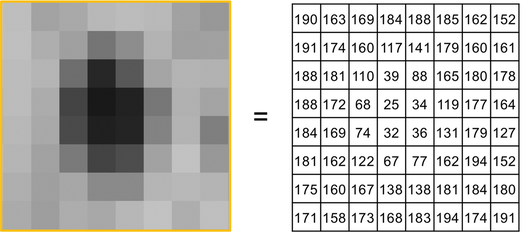
\includegraphics[width=0.5\linewidth]{Grayscale-image-expressed-in-a-matrix-of-numbers-that-computers-can-process-a-8-bit.png}
    \caption{Transformação de uma imagem em uma matriz²}
    \label{fig:enter-label}
\end{figure}

\subsection{Análise de Componentes Principais (PCA)}

A Análise de Componentes Principais é um método de redução de dimensionalidade frequentemente utilizado em conjuntos de dados com um número muito grande de variáveis. Com a aplicação desse processo, a quantidade de variáveis a serem analisadas é reduzida, de forma que seu processamento se torna bem mais simples. Para isso, a PCA é capaz de identificar as variáveis que melhor representam o dado como um todo e excluir apenas variáveis não tão significativas, fazendo com que, apesar da eliminação de valores, a perda de informação seja relativamente baixa em comparação à simplificação obtida.\\

\subsubsection{Padronização}

A primeira fase do processo de Análise de Componentes Principais refere-se à padronização dos dados, cujo objetivo é amenizar a diferença entre os registros e colocá-los na mesma escala. Dessa forma, cada variável contribui de forma relativamente equivalente para a análise.\\

Para isso, é subtraída de cada valor a média dos valores daquela variável e esse resultado é dividido pelo desvio-padrão desses registros, como mostrado abaixo:

\begin{align*}
    valor_{novo} = \frac{(valor_{antigo} - \textit{média})}{\textit{desvio padrão}}
\end{align*}
\\

Dessa forma, a distribuição dos dados é preservada, mas sua escala é alterada de modo a igualar sua média a 0 e a normalizar sua escala. Isso pode ser observado na figura 2.

\begin{figure}[h]
    \centering
    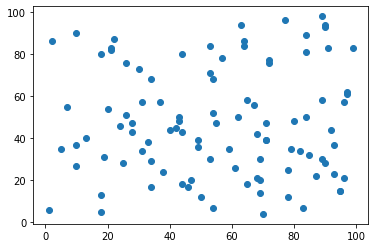
\includegraphics[width=0.4\linewidth]{Figure 2023-11-09 104557.png}
    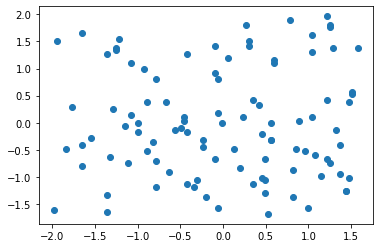
\includegraphics[width=0.4\linewidth]{Figure 2023-11-09 104605.png}
    \caption{Padronização dos dados}
    \label{fig:enter-label}
\end{figure}

\subsubsection{Cálculo da matriz de covariância}

O objetivo da matriz de covariância é estabelecer relações entre as variáveis da base de dados, de forma a identificar aquelas que são direta ou inversamente correlacionadas e aquelas que não têm relação umas com a outras.\\

Se uma covariância é positiva, então as variáveis são diretamente correlacionadas, ou seja, crescem ou decrescem juntas. Se for negativa, elas são inversamente correlacionadas, isto é, enquanto uma cresce, a outra decresce. Por fim, valores próximos de zero indicam ausência de correlação entre as variáveis. \\

Agora, suponhamos uma matriz de dados A com $m$ registros e $n$ variáveis, como indicado a seguir.

\[
A = 
\begin{bNiceMatrix}[first-col,first-row]
       & v_1    & v_2    & \cdots & v_n \\
r_1    & a_{11} & a_{12} & \cdots & a_{1n} \\
r_2    & a_{21} & a_{22} & \cdots & a_{2n} \\
\vdots & \vdots & \vdots & \ddots & \vdots \\
r_m    & a_{m1} & a_{m2} & \cdots & a_{mn}
\end{bNiceMatrix}
\]
\\

Para calcularmos as covariâncias entre as variáveis dessa matriz, precisamos fazer o produto interno entre cada par de variáveis, ou seja, entre todas as colunas dessa matriz. Para isso, basta fazermos $A^TA$ e obteremos a seguinte matriz de covariâncias:

\[
\left[ {\begin{array}{cccc}
    Cov(v_1, v_1) & Cov(v_1, v_2) & \cdots & Cov(v_1, v_n) \\
    Cov(v_2, v_1) & Cov(v_2, v_2) & \cdots & Cov(v_2, v_n) \\
    \vdots        & \vdots        & \ddots & \vdots     \\
    Cov(v_n, v_1) & Cov(v_n, v_2) & \cdots & Cov(v_n, v_n) \\
\end{array}} \right]
\]
\\

Dois pontos importantes sobre essa matriz:

\begin{itemize}
    \item A diagonal é composta pelas covariâncias de uma variável com ela mesmo. Por definição, esses valores representam a \textbf{variância} de cada variável.

    \item Devido ao fato de o produto interno ser comutativo ($u^Tv = v^Tu$), temos que $Cov(v_i, v_j) = Cov(v_j, v_i)$. Portanto, essa matriz é \textbf{simétrica}.
\end{itemize}

\subsubsection{Autovalores e autovetores da matriz de covariância}

Agora, vamos analisar essa matriz de covariância para ver que informações ela contém. \\

Os autovetores dessa matriz indicam as direções de maior variância do dado, enquanto que seus respectivos autovalores representam a variância na direção de seu autovetor. Com isso, podemos rankear os autovetores de acordo com seus autovalores de forma a descobrir as direções em que o dado mais varia e, portanto, mais significativas. Essas direções são as \textbf{componentes principais}. \\

Essas componentes são combinações lineares das variáveis originais, não tendo nenhum significado real para o dado. Apesar disso, podemos usá-las para simplificar nossa base, já que podemos desconsiderar as componentes principais de menores autovalores (ou seja, que compõem uma parcela pequena da variância do dado) e, assim, representar de forma mais simples a distribuição do dado. Além disso, devido ao fato de a matriz de covariância ser simétrica, esses autovetores são \textbf{ortogonais}, fazendo com que possamos formar com eles uma nova base ortogonal para os dados. \\

\subsubsection{Exemplo de uso}

Vamos aplicar esse procedimento a uma base de modelo para demonstrar suas etapas e seu funcionamento. Comecemos com o seguinte dado já normalizado:

\vspace{4cm}

\begin{figure}[h!]
    \centering
    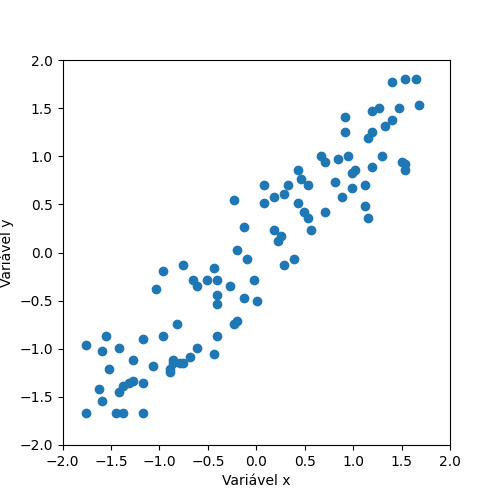
\includegraphics[width=0.4\linewidth]{Figure_3.png}
    \caption{Dado original}
    \label{fig:enter-label}
\end{figure}

Inicialmente, calculamos sua matriz de covariância e obtemos o seguinte resultado:

\[
\left[ {\begin{array}{cc}
    100 & 92.37568063 \\
    92.37568063 & 100 \\
\end{array}} \right]
\]
\\

A seguir, calculamos seus autovalores e autovetores:

\begin{equation*}
    \lambda_1 = 192,376
    \qquad
    x_1 =
    \left[
    \begin{array}{c}
         1 \\
         1
    \end{array}
    \right]
\end{equation*}
    
\begin{equation*}
    \lambda_2 = 7,624
    \qquad
    x_2 =
    \left[
    \begin{array}{c}
         -1 \\
         1
    \end{array}
    \right] \\
\end{equation*}
\\

Notemos que o autovalor do primeiro autovetor é bem mais significativo que o do primeiro. Assim, concluímos que a direção de $x_1$ é a de maior variância de todo o dado, enquanto que a de $x_2$ é a segunda maior. Além disso, é perceptível que esses dois autovetores são ortogonais, o que é lógico dado o fato de que a matriz de covariância é simétrica. \\

Dessa forma, conseguimos "separar" a variância total do dado entre as duas componentes principais obtidas por meio da comparação entre seus autovalores, ou seja, a proporção de cada um deles no somatório de todos os autovalores. Com isso, podemos gerar o seguinte gráfico:

\begin{figure}[h!]
    \centering
    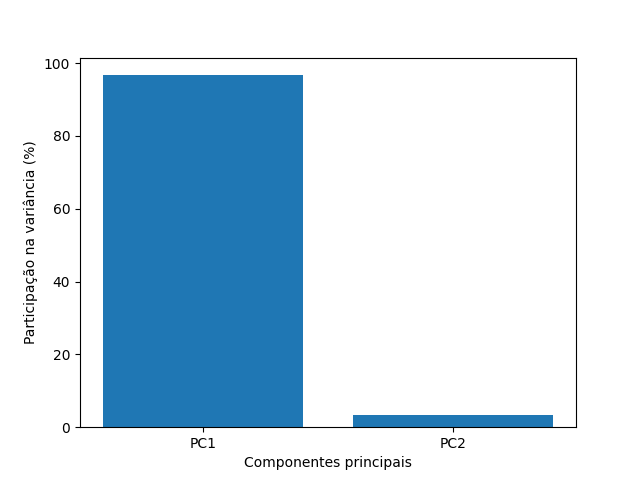
\includegraphics[width=0.4\linewidth]{Figure_5.png}
    \caption{Proporção de cada componente principal (PC) na variância do dado em porcentagem}
    \label{fig:enter-label}
\end{figure}

Podemos concluir que a direção do autovetor $x_1$ é responsável por quase toda a variância do dado. Se tivéssemos mais variáveis, obteríamos mais componentes principais, e poderíamos simplesmente desconsiderar as menos relevantes de modo a simplificar a análise dos dados. No entanto, nesse exemplo, esse não é o objetivo. \\

Agora, plotemos no gráfico nossos autovetores para entendê-los melhor.

\begin{figure}[h!]
    \centering
    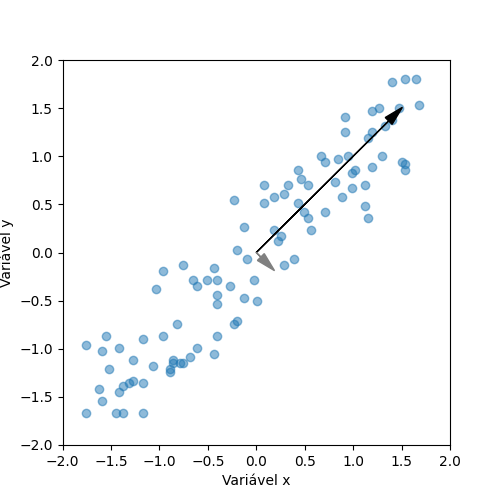
\includegraphics[width=0.4\linewidth]{Figure_4.png}
    \caption{Dado original e suas direções de variância}
    \label{fig:enter-label}
\end{figure}

Nessa figura, $x_1$ está representado em preto e $x_2$ em cinza. É visível o fato de a direção do vetor preto ser a direção de maior variância do dado. \\

Por fim, podemos agora projetar esses dados no espaço gerado pelas componentes principais para obter sua nova distribuição. Para isso, chamando a matriz de autovetores da matriz de covariância de $autovetores_{cov}$, basta fazermos:

\begin{align*}
    dado_{novo} = (autovetores_{cov})^Tdado_{original}
\end{align*}

Fazendo isso com nossa base, obtemos, finalmente, a seguinte nova distribuição:

\begin{figure}[h!]
    \centering
    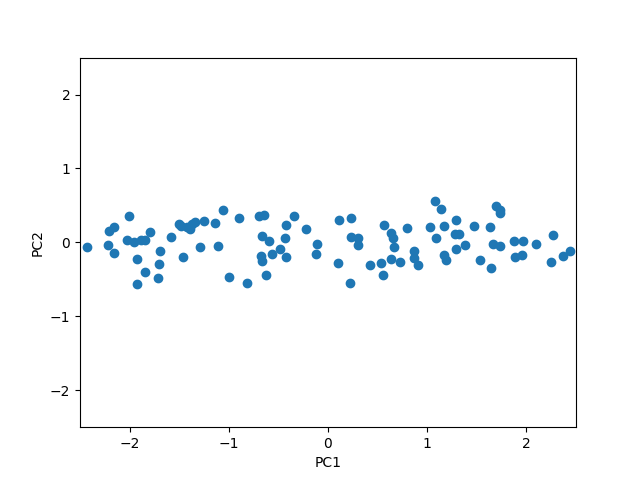
\includegraphics[width=0.4\linewidth]{Figure_6.png}
    \caption{Novo dado}
    \label{fig:enter-label}
\end{figure}

Com isso, conseguimos uma simplificação do dado fazendo com que seu principal eixo de variação seja o eixo horizontal e não mais uma direção genérica. \\

Vale ressaltar que o principal objetivo do método do PCA é a redução de dimensionalidade do dado. Nesse exemplo, apesar de aproximarmos nosso dado de algo unidimensional, não o fizemos realmente. A ideia geral desse processo é transformar uma base de dados de 50 variáveis, por exemplo, em uma base de 10, com essas novas 10 variáveis sendo combinações das variáveis originais que representem a maior parte da variação do dado. No entanto, isso não era muito prático de se mostrar aqui de uma forma simples (infelizmente, ainda não descobrimos como plotar 50 variáveis). \\

\subsection{Eigenfaces}
Seguindo a ideia da análise de componentes principais, podemos seguir com o cálculo das eigenfaces, que nada mais é do que uma base ortogonal do espaço das "faces". Cada imagem retratada por um vetor é um ponto no espaço $R^{N_{1}\times N_{2}}$ no qual a dimensão da imagem é ${N_{1}\times N_{2}}$. Como ${N_{1}\times N_{2}}$ acaba sendo um número muito grande, procuraremos os principais componentes desse espaço, ou seja, os vetores que mais explicam a variação do dado.\\

Supomos que temos uma sequência de M fotos de ${N_{1}\times N_{2}}$. Por consequência, temos uma matriz ${N_{1}\times N_{2}}$ por M, na qual cada imagem é representado pela coluna $\Gamma_{i}$. Para seguir com a análise da PCA. calcularemos a imagem média $\Psi$ do dataset:\\
\begin{align*}
    \Psi = \frac{1}{M}\sum_{i=1}^{M}\Gamma_{i}
\end{align*} \\

E, para achar a base de dados centralizados, diminuiremos cada vetor do vetor médio e colocaremos todos numa matriz:\\

\begin{gather*}
    \Phi_{i} = \Gamma_{i}-\Psi \\
    A = [\Phi_{1}, \Phi_{2}, ..., \Phi_{M}]
\end{gather*}\\

Agora buscaremos um conjunto de vetores ortonormais de forma que 
\begin{gather*}
    \lambda_{k} = \frac{1}{M}\sum_{i=1}^{M}(u_{k}^T\Phi_{i})^2,
\end{gather*}\\
no qual temos a restrição de $u_{k}$ ser ortonormal.
Os vetores $u_{k}$ são os autovetores e os elementos $\lambda_{k}$ são os autovalores da matriz de covariância, definida como:\\
\begin{gather*}
    C = \frac{1}{M}\sum_{i=1}^{M}(\Phi_{i} \Phi_{i}^T)\\
    C = AA^T,
\end{gather*}\\
na qual A é a matriz com autovetores. 
No entanto, temos um problema com a quantidade de termos necessários para se calcular. A matriz C é de tamanho $(N_{1}\times N_{2})^2 \times (N_{1}\times N_{2})^2$, e como estamos tratando de vetores com um N muito grande, calcular uma matriz do tamanho de C seria algo muito custoso. No entanto, podemos utilizar o fato de que os autovalores de $AA^T$
são os mesmos de $A^TA$, como mostrado abaixo:
\begin{gather*}
    A^TAv_{i} = \lambda v_{i}\\
    AA^TAv_{i} = \lambda Av_{i}\\
    (AA^T)Av_{i} = (\lambda) Av_{i}
\end{gather*}\\

Como consequência, ficamos com a matriz $A^TA$ muito mais simples de se calcular, pois no fim teremos uma matriz $M \times M$, com muito menos entradas. Reduzimos, assim, a quantidade de cálculos necessários de um número muito grande para M. Ficamos então com a matriz

\begin{gather*}
    L = A^TA\\
    \quad \text{onde}\quad L_{mn} = \Phi_{i}^T \Phi_{i}.
\end{gather*}\\

Chame os autovetores dessa matriz de $v_{i}$. Esses vetores formam as combinações lineares das N imagens escolhidas e, portanto, podemos voltar para encontrar os vetores $u$ previamente especificados de acordo com:

\begin{gather*}
    u_{l}= \sum_{i=1}^{N}v_{lk}\Phi_{k}  \quad     \quad   l = 1,2 ..., M.
\end{gather*}

\section{Aplicando eigenfaces para reconhecimento facial}

Feita a explicação teórica, vamos à aplicação prática. Nesse projeto,
temos 20 imagens do artista Will Smith e outras 20 da cantora Taylor
Swift. Nosso objetivo é verificar se o método de eigenfaces é capaz de
distingui-los e indentificá-los.\\

Antes de começarmos, um adendo: infelizmente, nessa aplicação
computacional, não conseguimos utilizar a matriz dos dados com os
registros nas colunas como explicado anteriormente. Em vez disso,
tivemos que fazer das imagens vetores-linha. Tirando essa alteração,
todo o restante do processo é semelhante ao descrito na parte teórica.\\

Inicialmente, importamos as bibliotecas~necessárias.

    \begin{tcolorbox}[breakable, size=fbox, boxrule=1pt, pad at break*=1mm,colback=cellbackground, colframe=cellborder]
\prompt{In}{incolor}{15}{\boxspacing}
\begin{Verbatim}[commandchars=\\\{\}]
\PY{k+kn}{import} \PY{n+nn}{numpy} \PY{k}{as} \PY{n+nn}{np}
\PY{k+kn}{import} \PY{n+nn}{pandas} \PY{k}{as} \PY{n+nn}{pd}
\PY{k+kn}{import} \PY{n+nn}{matplotlib}\PY{n+nn}{.}\PY{n+nn}{pyplot} \PY{k}{as} \PY{n+nn}{plt}
\PY{k+kn}{import} \PY{n+nn}{cv2}
\PY{k+kn}{import} \PY{n+nn}{os}
\end{Verbatim}
\end{tcolorbox}

    Para que o método funcione, é necessário que todas as imagens possuam as
mesmas dimensões. Dessa forma, optamos por figuras de tamanho 195x231.

    \begin{tcolorbox}[breakable, size=fbox, boxrule=1pt, pad at break*=1mm,colback=cellbackground, colframe=cellborder]
\prompt{In}{incolor}{16}{\boxspacing}
\begin{Verbatim}[commandchars=\\\{\}]
\PY{n}{altura\PYZus{}imagem} \PY{o}{=} \PY{l+m+mi}{231}
\PY{n}{comprimento} \PY{o}{=} \PY{l+m+mi}{195}
\end{Verbatim}
\end{tcolorbox}

    A seguir, fizemos a leituras das imagens e as convertemos em uma matriz
tridimensional (cada imagem é uma matriz bidimensional e sua composição
adiciona uma terceira dimensão).

    \begin{tcolorbox}[breakable, size=fbox, boxrule=1pt, pad at break*=1mm,colback=cellbackground, colframe=cellborder]
\prompt{In}{incolor}{17}{\boxspacing}
\begin{Verbatim}[commandchars=\\\{\}]
\PY{c+c1}{\PYZsh{} Criando o path para onde as imagens estão}
\PY{n}{famousim} \PY{o}{=} \PY{l+s+s2}{\PYZdq{}}\PY{l+s+s2}{imagens\PYZus{}artistas/}\PY{l+s+s2}{\PYZdq{}}
\PY{c+c1}{\PYZsh{} Criando uma lista para adicionar as imagens}
\PY{n}{famous\PYZus{}images} \PY{o}{=} \PY{p}{[}\PY{p}{]}

\PY{c+c1}{\PYZsh{} Fazendo um loop for para iterar sobre todas as imagens}
\PY{k}{for} \PY{n}{folder} \PY{o+ow}{in} \PY{p}{(}\PY{n}{os}\PY{o}{.}\PY{n}{listdir}\PY{p}{(}\PY{n}{famousim}\PY{p}{)}\PY{p}{)}\PY{p}{:}
    \PY{n}{folder\PYZus{}path} \PY{o}{=} \PY{n}{os}\PY{o}{.}\PY{n}{path}\PY{o}{.}\PY{n}{join}\PY{p}{(}\PY{n}{famousim}\PY{p}{,} \PY{n}{folder}\PY{p}{)}
    \PY{k}{for} \PY{n}{image} \PY{o+ow}{in} \PY{p}{(}\PY{n}{os}\PY{o}{.}\PY{n}{listdir}\PY{p}{(}\PY{n}{folder\PYZus{}path}\PY{p}{)}\PY{p}{)}\PY{p}{:}
        \PY{c+c1}{\PYZsh{} Adicionando o path com cada imagem para termos o arquivo das imagens}
        \PY{n}{path} \PY{o}{=} \PY{n}{os}\PY{o}{.}\PY{n}{path}\PY{o}{.}\PY{n}{join}\PY{p}{(}\PY{n}{famousim}\PY{p}{,} \PY{n}{folder} \PY{p}{,}\PY{n}{image}\PY{p}{)}
        \PY{c+c1}{\PYZsh{} Lendo a imagem}
        \PY{n}{img} \PY{o}{=} \PY{n}{cv2}\PY{o}{.}\PY{n}{imread}\PY{p}{(}\PY{n}{path}\PY{p}{)}
        \PY{c+c1}{\PYZsh{} Convertendo a imagem para preto e branco }
        \PY{n}{img} \PY{o}{=} \PY{n}{cv2}\PY{o}{.}\PY{n}{cvtColor}\PY{p}{(}\PY{n}{img}\PY{p}{,} \PY{n}{cv2}\PY{o}{.}\PY{n}{COLOR\PYZus{}BGR2GRAY}\PY{p}{)}
        \PY{c+c1}{\PYZsh{} Adicionando a imagem na lista}
        \PY{n}{famous\PYZus{}images}\PY{o}{.}\PY{n}{append}\PY{p}{(}\PY{n}{img}\PY{p}{)}

\PY{c+c1}{\PYZsh{} Transformando a lista num array}
\PY{n}{famous\PYZus{}images\PYZus{}np} \PY{o}{=} \PY{n}{np}\PY{o}{.}\PY{n}{array}\PY{p}{(}\PY{n}{famous\PYZus{}images}\PY{p}{)}
\end{Verbatim}
\end{tcolorbox}

    Vamos dar uma olhada nas nossas imagens.

    \begin{tcolorbox}[breakable, size=fbox, boxrule=1pt, pad at break*=1mm,colback=cellbackground, colframe=cellborder]
\prompt{In}{incolor}{18}{\boxspacing}
\begin{Verbatim}[commandchars=\\\{\}]
\PY{c+c1}{\PYZsh{} Plotando as imagens}
\PY{n}{count} \PY{o}{=} \PY{l+m+mi}{0}
\PY{n}{fig}\PY{p}{,} \PY{n}{ax} \PY{o}{=} \PY{n}{plt}\PY{o}{.}\PY{n}{subplots}\PY{p}{(}\PY{l+m+mi}{5}\PY{p}{,} \PY{l+m+mi}{8}\PY{p}{,} \PY{n}{figsize}\PY{o}{=}\PY{p}{(}\PY{l+m+mi}{10}\PY{p}{,} \PY{l+m+mi}{10}\PY{p}{)}\PY{p}{)}
\PY{k}{for} \PY{n}{linha} \PY{o+ow}{in} \PY{n+nb}{range}\PY{p}{(}\PY{l+m+mi}{5}\PY{p}{)}\PY{p}{:}
    \PY{k}{for} \PY{n}{coluna} \PY{o+ow}{in} \PY{n+nb}{range}\PY{p}{(}\PY{l+m+mi}{8}\PY{p}{)}\PY{p}{:}
        \PY{n}{ax}\PY{p}{[}\PY{n}{linha}\PY{p}{,}\PY{n}{coluna}\PY{p}{]}\PY{o}{.}\PY{n}{imshow}\PY{p}{(}\PY{n}{famous\PYZus{}images\PYZus{}np}\PY{p}{[}\PY{n}{count}\PY{p}{]}\PY{p}{,} \PY{n}{cmap}\PY{o}{=}\PY{l+s+s1}{\PYZsq{}}\PY{l+s+s1}{gray}\PY{l+s+s1}{\PYZsq{}}\PY{p}{)}
        \PY{n}{count} \PY{o}{+}\PY{o}{=} \PY{l+m+mi}{1}
        \PY{n}{ax}\PY{p}{[}\PY{n}{linha}\PY{p}{,} \PY{n}{coluna}\PY{p}{]}\PY{o}{.}\PY{n}{set\PYZus{}xticks}\PY{p}{(}\PY{p}{[}\PY{p}{]}\PY{p}{)}
        \PY{n}{ax}\PY{p}{[}\PY{n}{linha}\PY{p}{,} \PY{n}{coluna}\PY{p}{]}\PY{o}{.}\PY{n}{set\PYZus{}yticks}\PY{p}{(}\PY{p}{[}\PY{p}{]}\PY{p}{)}
        \PY{n}{ax}\PY{p}{[}\PY{n}{linha}\PY{p}{,} \PY{n}{coluna}\PY{p}{]}\PY{o}{.}\PY{n}{set\PYZus{}xticklabels}\PY{p}{(}\PY{p}{[}\PY{p}{]}\PY{p}{)}
        \PY{n}{ax}\PY{p}{[}\PY{n}{linha}\PY{p}{,} \PY{n}{coluna}\PY{p}{]}\PY{o}{.}\PY{n}{set\PYZus{}yticklabels}\PY{p}{(}\PY{p}{[}\PY{p}{]}\PY{p}{)}
        \PY{n}{ax}\PY{p}{[}\PY{n}{linha}\PY{p}{,} \PY{n}{coluna}\PY{p}{]}\PY{o}{.}\PY{n}{set\PYZus{}xlabel}\PY{p}{(}\PY{l+s+s1}{\PYZsq{}}\PY{l+s+s1}{\PYZsq{}}\PY{p}{)}
        \PY{n}{ax}\PY{p}{[}\PY{n}{linha}\PY{p}{,} \PY{n}{coluna}\PY{p}{]}\PY{o}{.}\PY{n}{set\PYZus{}ylabel}\PY{p}{(}\PY{l+s+s1}{\PYZsq{}}\PY{l+s+s1}{\PYZsq{}}\PY{p}{)}
\end{Verbatim}
\end{tcolorbox}

    \begin{center}
    \adjustimage{max size={0.8\linewidth}{0.8\paperheight}}{output_8_0.png}
    \end{center}
    { \hspace*{\fill} \\}
    
    Agora, transformamos essa matriz tridimensional em uma matriz
bidimensional convertendo as matrizes de cada imagem para um único
vetor-linha extremamente comprido. Após isso, calculamos a face média.

    \begin{tcolorbox}[breakable, size=fbox, boxrule=1pt, pad at break*=1mm,colback=cellbackground, colframe=cellborder]
\prompt{In}{incolor}{19}{\boxspacing}
\begin{Verbatim}[commandchars=\\\{\}]
\PY{c+c1}{\PYZsh{} Cada imagem está armazenada em 3 dimensões, cada foto está numa lista, e cada lista é uma lista de listas.}
\PY{c+c1}{\PYZsh{} Vamos transformar a imagem num vetor coluna muito grande.}
\PY{n}{train\PYZus{}famous\PYZus{}np\PYZus{}matrix} \PY{o}{=} \PY{n}{famous\PYZus{}images\PYZus{}np}\PY{o}{.}\PY{n}{reshape}\PY{p}{(}\PY{n}{famous\PYZus{}images\PYZus{}np}\PY{o}{.}\PY{n}{shape}\PY{p}{[}\PY{l+m+mi}{0}\PY{p}{]}\PY{p}{,} \PY{n}{famous\PYZus{}images\PYZus{}np}\PY{o}{.}\PY{n}{shape}\PY{p}{[}\PY{l+m+mi}{1}\PY{p}{]}\PY{o}{*}\PY{n}{famous\PYZus{}images\PYZus{}np}\PY{o}{.}\PY{n}{shape}\PY{p}{[}\PY{l+m+mi}{2}\PY{p}{]}\PY{p}{)}
\PY{c+c1}{\PYZsh{} Calculamos a face média}
\PY{n}{mean\PYZus{}train\PYZus{}face} \PY{o}{=} \PY{n}{np}\PY{o}{.}\PY{n}{mean}\PY{p}{(}\PY{n}{train\PYZus{}famous\PYZus{}np\PYZus{}matrix}\PY{p}{,} \PY{n}{axis}\PY{o}{=}\PY{l+m+mi}{0}\PY{p}{)}
\PY{c+c1}{\PYZsh{} Criamos uma matriz subtraindo a face média}
\PY{n}{centered\PYZus{}train\PYZus{}face} \PY{o}{=} \PY{n}{train\PYZus{}famous\PYZus{}np\PYZus{}matrix} \PY{o}{\PYZhy{}} \PY{n}{mean\PYZus{}train\PYZus{}face}

\PY{c+c1}{\PYZsh{} Mostrando a face média}
\PY{n}{plt}\PY{o}{.}\PY{n}{figure}\PY{p}{(}\PY{p}{)}
\PY{n}{plt}\PY{o}{.}\PY{n}{imshow}\PY{p}{(}\PY{n}{mean\PYZus{}train\PYZus{}face}\PY{o}{.}\PY{n}{reshape}\PY{p}{(}\PY{n}{altura\PYZus{}imagem}\PY{p}{,}\PY{n}{comprimento}\PY{p}{)}\PY{p}{,} \PY{n}{cmap}\PY{o}{=}\PY{l+s+s1}{\PYZsq{}}\PY{l+s+s1}{gray}\PY{l+s+s1}{\PYZsq{}}\PY{p}{)}
\end{Verbatim}
\end{tcolorbox}

            \begin{tcolorbox}[breakable, size=fbox, boxrule=.5pt, pad at break*=1mm, opacityfill=0]
\prompt{Out}{outcolor}{19}{\boxspacing}
\begin{Verbatim}[commandchars=\\\{\}]
<matplotlib.image.AxesImage at 0x15621f964a0>
\end{Verbatim}
\end{tcolorbox}
        
    \begin{center}
    \adjustimage{max size={0.5\linewidth}{0.5\paperheight}}{output_10_1.png}
    \end{center}
    { \hspace*{\fill} \\}
    
    A seguir, calculamos a decomposição SVD dessa matriz.

    \begin{tcolorbox}[breakable, size=fbox, boxrule=1pt, pad at break*=1mm,colback=cellbackground, colframe=cellborder]
\prompt{In}{incolor}{20}{\boxspacing}
\begin{Verbatim}[commandchars=\\\{\}]
\PY{c+c1}{\PYZsh{} Decompomdo a matriz em SVD}
\PY{n}{U\PYZus{}Face\PYZus{}Famous}\PY{p}{,} \PY{n}{D\PYZus{}Face\PYZus{}Famous}\PY{p}{,} \PY{n}{V\PYZus{}Face\PYZus{}Famous} \PY{o}{=} \PY{n}{np}\PY{o}{.}\PY{n}{linalg}\PY{o}{.}\PY{n}{svd}\PY{p}{(}\PY{n}{centered\PYZus{}train\PYZus{}face}\PY{p}{,} \PY{n}{full\PYZus{}matrices}\PY{o}{=}\PY{k+kc}{False}\PY{p}{)}
\end{Verbatim}
\end{tcolorbox}

    Vamos selecionar as 12 primeiras componentes principais e plotar suas
eigenfaces.

    \begin{tcolorbox}[breakable, size=fbox, boxrule=1pt, pad at break*=1mm,colback=cellbackground, colframe=cellborder]
\prompt{In}{incolor}{21}{\boxspacing}
\begin{Verbatim}[commandchars=\\\{\}]
\PY{c+c1}{\PYZsh{} Vamos obter a quantidade de componentes que queremos de nossa matriz.}
\PY{n}{C\PYZus{}Faces\PYZus{}TRAIN} \PY{o}{=} \PY{n}{V\PYZus{}Face\PYZus{}Famous}\PY{p}{[}\PY{p}{:}\PY{l+m+mi}{12}\PY{p}{]}
\PY{n}{eigen\PYZus{}faces\PYZus{}train} \PY{o}{=} \PY{n}{C\PYZus{}Faces\PYZus{}TRAIN}\PY{o}{.}\PY{n}{reshape}\PY{p}{(}\PY{p}{(}\PY{o}{\PYZhy{}}\PY{l+m+mi}{1}\PY{p}{,} \PY{n}{altura\PYZus{}imagem}\PY{p}{,} \PY{n}{comprimento}\PY{p}{)}\PY{p}{)}
\end{Verbatim}
\end{tcolorbox}

    \begin{tcolorbox}[breakable, size=fbox, boxrule=1pt, pad at break*=1mm,colback=cellbackground, colframe=cellborder]
\prompt{In}{incolor}{22}{\boxspacing}
\begin{Verbatim}[commandchars=\\\{\}]
\PY{n}{count} \PY{o}{=} \PY{l+m+mi}{0}
\PY{n}{fig}\PY{p}{,} \PY{n}{ax} \PY{o}{=} \PY{n}{plt}\PY{o}{.}\PY{n}{subplots}\PY{p}{(}\PY{l+m+mi}{3}\PY{p}{,} \PY{l+m+mi}{4}\PY{p}{,} \PY{n}{figsize}\PY{o}{=}\PY{p}{(}\PY{l+m+mi}{10}\PY{p}{,} \PY{l+m+mi}{10}\PY{p}{)}\PY{p}{)}
\PY{k}{for} \PY{n}{linha} \PY{o+ow}{in} \PY{n+nb}{range}\PY{p}{(}\PY{l+m+mi}{3}\PY{p}{)}\PY{p}{:}
    \PY{k}{for} \PY{n}{coluna} \PY{o+ow}{in} \PY{n+nb}{range}\PY{p}{(}\PY{l+m+mi}{4}\PY{p}{)}\PY{p}{:}
        \PY{n}{ax}\PY{p}{[}\PY{n}{linha}\PY{p}{,}\PY{n}{coluna}\PY{p}{]}\PY{o}{.}\PY{n}{imshow}\PY{p}{(}\PY{n}{eigen\PYZus{}faces\PYZus{}train}\PY{p}{[}\PY{n}{count}\PY{p}{]}\PY{p}{,} \PY{n}{cmap}\PY{o}{=}\PY{l+s+s1}{\PYZsq{}}\PY{l+s+s1}{gray}\PY{l+s+s1}{\PYZsq{}}\PY{p}{)}
        \PY{n}{count} \PY{o}{+}\PY{o}{=} \PY{l+m+mi}{1}
        \PY{n}{ax}\PY{p}{[}\PY{n}{linha}\PY{p}{,} \PY{n}{coluna}\PY{p}{]}\PY{o}{.}\PY{n}{set\PYZus{}xticks}\PY{p}{(}\PY{p}{[}\PY{p}{]}\PY{p}{)}
        \PY{n}{ax}\PY{p}{[}\PY{n}{linha}\PY{p}{,} \PY{n}{coluna}\PY{p}{]}\PY{o}{.}\PY{n}{set\PYZus{}yticks}\PY{p}{(}\PY{p}{[}\PY{p}{]}\PY{p}{)}
        \PY{n}{ax}\PY{p}{[}\PY{n}{linha}\PY{p}{,} \PY{n}{coluna}\PY{p}{]}\PY{o}{.}\PY{n}{set\PYZus{}xticklabels}\PY{p}{(}\PY{p}{[}\PY{p}{]}\PY{p}{)}
        \PY{n}{ax}\PY{p}{[}\PY{n}{linha}\PY{p}{,} \PY{n}{coluna}\PY{p}{]}\PY{o}{.}\PY{n}{set\PYZus{}yticklabels}\PY{p}{(}\PY{p}{[}\PY{p}{]}\PY{p}{)}
        \PY{n}{ax}\PY{p}{[}\PY{n}{linha}\PY{p}{,} \PY{n}{coluna}\PY{p}{]}\PY{o}{.}\PY{n}{set\PYZus{}xlabel}\PY{p}{(}\PY{l+s+s1}{\PYZsq{}}\PY{l+s+s1}{\PYZsq{}}\PY{p}{)}
        \PY{n}{ax}\PY{p}{[}\PY{n}{linha}\PY{p}{,} \PY{n}{coluna}\PY{p}{]}\PY{o}{.}\PY{n}{set\PYZus{}ylabel}\PY{p}{(}\PY{l+s+s1}{\PYZsq{}}\PY{l+s+s1}{\PYZsq{}}\PY{p}{)}
\end{Verbatim}
\end{tcolorbox}

    \begin{center}
    \adjustimage{max size={0.8\linewidth}{0.8\paperheight}}{output_15_0.png}
    \end{center}
    { \hspace*{\fill} \\}
    
    Vamos dar uma olhada em nossas imagens agora centralizadas (subtraídas a
média).

    \begin{tcolorbox}[breakable, size=fbox, boxrule=1pt, pad at break*=1mm,colback=cellbackground, colframe=cellborder]
\prompt{In}{incolor}{23}{\boxspacing}
\begin{Verbatim}[commandchars=\\\{\}]
\PY{n}{count} \PY{o}{=} \PY{l+m+mi}{0}
\PY{n}{fig}\PY{p}{,} \PY{n}{ax} \PY{o}{=} \PY{n}{plt}\PY{o}{.}\PY{n}{subplots}\PY{p}{(}\PY{l+m+mi}{5}\PY{p}{,} \PY{l+m+mi}{8}\PY{p}{,} \PY{n}{figsize}\PY{o}{=}\PY{p}{(}\PY{l+m+mi}{10}\PY{p}{,} \PY{l+m+mi}{10}\PY{p}{)}\PY{p}{)}
\PY{k}{for} \PY{n}{linha} \PY{o+ow}{in} \PY{n+nb}{range}\PY{p}{(}\PY{l+m+mi}{5}\PY{p}{)}\PY{p}{:}
    \PY{k}{for} \PY{n}{coluna} \PY{o+ow}{in} \PY{n+nb}{range}\PY{p}{(}\PY{l+m+mi}{8}\PY{p}{)}\PY{p}{:}
        \PY{n}{ax}\PY{p}{[}\PY{n}{linha}\PY{p}{,}\PY{n}{coluna}\PY{p}{]}\PY{o}{.}\PY{n}{imshow}\PY{p}{(}\PY{n}{centered\PYZus{}train\PYZus{}face}\PY{p}{[}\PY{n}{count}\PY{p}{]}\PY{o}{.}\PY{n}{reshape}\PY{p}{(}\PY{n}{altura\PYZus{}imagem}\PY{p}{,}\PY{n}{comprimento}\PY{p}{)}\PY{p}{,} \PY{n}{cmap}\PY{o}{=}\PY{l+s+s1}{\PYZsq{}}\PY{l+s+s1}{gray}\PY{l+s+s1}{\PYZsq{}}\PY{p}{)}
        \PY{n}{count} \PY{o}{+}\PY{o}{=} \PY{l+m+mi}{1}
        \PY{n}{ax}\PY{p}{[}\PY{n}{linha}\PY{p}{,} \PY{n}{coluna}\PY{p}{]}\PY{o}{.}\PY{n}{set\PYZus{}xticks}\PY{p}{(}\PY{p}{[}\PY{p}{]}\PY{p}{)}
        \PY{n}{ax}\PY{p}{[}\PY{n}{linha}\PY{p}{,} \PY{n}{coluna}\PY{p}{]}\PY{o}{.}\PY{n}{set\PYZus{}yticks}\PY{p}{(}\PY{p}{[}\PY{p}{]}\PY{p}{)}
        \PY{n}{ax}\PY{p}{[}\PY{n}{linha}\PY{p}{,} \PY{n}{coluna}\PY{p}{]}\PY{o}{.}\PY{n}{set\PYZus{}xticklabels}\PY{p}{(}\PY{p}{[}\PY{p}{]}\PY{p}{)}
        \PY{n}{ax}\PY{p}{[}\PY{n}{linha}\PY{p}{,} \PY{n}{coluna}\PY{p}{]}\PY{o}{.}\PY{n}{set\PYZus{}yticklabels}\PY{p}{(}\PY{p}{[}\PY{p}{]}\PY{p}{)}
        \PY{n}{ax}\PY{p}{[}\PY{n}{linha}\PY{p}{,} \PY{n}{coluna}\PY{p}{]}\PY{o}{.}\PY{n}{set\PYZus{}xlabel}\PY{p}{(}\PY{l+s+s1}{\PYZsq{}}\PY{l+s+s1}{\PYZsq{}}\PY{p}{)}
        \PY{n}{ax}\PY{p}{[}\PY{n}{linha}\PY{p}{,} \PY{n}{coluna}\PY{p}{]}\PY{o}{.}\PY{n}{set\PYZus{}ylabel}\PY{p}{(}\PY{l+s+s1}{\PYZsq{}}\PY{l+s+s1}{\PYZsq{}}\PY{p}{)}
\end{Verbatim}
\end{tcolorbox}

    \begin{center}
    \adjustimage{max size={0.9\linewidth}{0.9\paperheight}}{output_17_0.png}
    \end{center}
    { \hspace*{\fill} \\}
    
    A seguir, vamos analisar a variância cumulativa das 40 componentes
principais. Desse modo, podemos considerar apenas as mais relevantes a
fim de simplificar a análise do dado.

    \begin{tcolorbox}[breakable, size=fbox, boxrule=1pt, pad at break*=1mm,colback=cellbackground, colframe=cellborder]
\prompt{In}{incolor}{24}{\boxspacing}
\begin{Verbatim}[commandchars=\\\{\}]
\PY{c+c1}{\PYZsh{} O quanto cada autovalor representa do dado?}

\PY{c+c1}{\PYZsh{} Somando todos os autovalores}
\PY{n}{sum\PYZus{}all} \PY{o}{=} \PY{n+nb}{sum}\PY{p}{(}\PY{n}{D\PYZus{}Face\PYZus{}Famous}\PY{p}{)}
\PY{c+c1}{\PYZsh{} Transformando o array com os autovalores numa soma cumulativa}
\PY{n}{cummulative} \PY{o}{=} \PY{p}{(}\PY{n}{np}\PY{o}{.}\PY{n}{cumsum}\PY{p}{(}\PY{n}{D\PYZus{}Face\PYZus{}Famous}\PY{p}{)}\PY{o}{.}\PY{n}{round}\PY{p}{(}\PY{l+m+mi}{2}\PY{p}{)}\PY{p}{)}\PY{o}{*}\PY{l+m+mi}{100}
\PY{c+c1}{\PYZsh{} Vendo quanto representa do total}
\PY{n}{percentage} \PY{o}{=} \PY{n}{cummulative}\PY{o}{/}\PY{n}{sum\PYZus{}all}

\PY{c+c1}{\PYZsh{} Plotando o gráfico}
\PY{n}{plt}\PY{o}{.}\PY{n}{bar}\PY{p}{(}\PY{n+nb}{range}\PY{p}{(}\PY{n+nb}{len}\PY{p}{(}\PY{n}{percentage}\PY{p}{)}\PY{p}{)}\PY{p}{,} \PY{n}{percentage}\PY{p}{,} \PY{n}{color}\PY{o}{=}\PY{l+s+s1}{\PYZsq{}}\PY{l+s+s1}{blue}\PY{l+s+s1}{\PYZsq{}}\PY{p}{,} \PY{n}{alpha}\PY{o}{=}\PY{l+m+mf}{0.7}\PY{p}{)}
\PY{n}{plt}\PY{o}{.}\PY{n}{title}\PY{p}{(}\PY{l+s+s2}{\PYZdq{}}\PY{l+s+s2}{Gráfico de variância por quantidade de PCA}\PY{l+s+s2}{\PYZsq{}}\PY{l+s+s2}{s}\PY{l+s+s2}{\PYZdq{}}\PY{p}{)}
\PY{n}{plt}\PY{o}{.}\PY{n}{xlabel}\PY{p}{(}\PY{l+s+s2}{\PYZdq{}}\PY{l+s+s2}{Quantidade de PCA}\PY{l+s+s2}{\PYZsq{}}\PY{l+s+s2}{s}\PY{l+s+s2}{\PYZdq{}}\PY{p}{)}
\PY{n}{plt}\PY{o}{.}\PY{n}{ylabel}\PY{p}{(}\PY{l+s+s2}{\PYZdq{}}\PY{l+s+si}{\PYZpc{} d}\PY{l+s+s2}{e explicação do dado}\PY{l+s+s2}{\PYZdq{}}\PY{p}{)}
\end{Verbatim}
\end{tcolorbox}

            \begin{tcolorbox}[breakable, size=fbox, boxrule=.5pt, pad at break*=1mm, opacityfill=0]
\prompt{Out}{outcolor}{24}{\boxspacing}
\begin{Verbatim}[commandchars=\\\{\}]
Text(0, 0.5, '\% de explicação do dado')
\end{Verbatim}
\end{tcolorbox}
        
    \begin{center}
    \adjustimage{max size={0.6\linewidth}{0.6\paperheight}}{output_19_1.png}
    \end{center}
    { \hspace*{\fill} \\}
    
    Podemos observar que as 20 primeiras componentes, ou seja, metade do
conjunto, é capaz de representar aproximadamente 70\% do dado. No
entanto, para fins lúdicos, utilizaremos a seguir apenas as 2 primeiras
a fim de ser possível plotá-las em um gráfico. Apesar de não serem tão
precisas, elas já representam 15\% da variação do dado, sendo suficiente
para nosso propósito.

    \begin{tcolorbox}[breakable, size=fbox, boxrule=1pt, pad at break*=1mm,colback=cellbackground, colframe=cellborder]
\prompt{In}{incolor}{25}{\boxspacing}
\begin{Verbatim}[commandchars=\\\{\}]
\PY{c+c1}{\PYZsh{} Nossa ideia agora, será pegar os dois principais componentes encontradas pelo PCA e então plotar as nossas imagens nesse subespaço}
\PY{n}{dois\PYZus{}maiores\PYZus{}PCAs} \PY{o}{=} \PY{n}{V\PYZus{}Face\PYZus{}Famous}\PY{p}{[}\PY{p}{:}\PY{l+m+mi}{2}\PY{p}{]}

\PY{c+c1}{\PYZsh{} Criando a lista o qual terão as coordenadas das imagens que já trainamos o nosso dado}
\PY{n}{coordinates} \PY{o}{=} \PY{p}{[}\PY{p}{]}

\PY{c+c1}{\PYZsh{} Fazendo um loop for para adicionar todas as imagens nessa lista}
\PY{k}{for} \PY{n}{img} \PY{o+ow}{in} \PY{n}{centered\PYZus{}train\PYZus{}face}\PY{p}{:}
    \PY{c+c1}{\PYZsh{} Fazendo o produto interno para achar a projeção de cada face no espaço das duas principais componentes.}
    \PY{n}{coordinates\PYZus{}xy} \PY{o}{=} \PY{n}{np}\PY{o}{.}\PY{n}{dot}\PY{p}{(}\PY{n}{dois\PYZus{}maiores\PYZus{}PCAs}\PY{p}{,} \PY{n}{img}\PY{p}{)}
    \PY{c+c1}{\PYZsh{} Adicionando na lista}
    \PY{n}{coordinates}\PY{o}{.}\PY{n}{append}\PY{p}{(}\PY{n}{coordinates\PYZus{}xy}\PY{p}{)}
\end{Verbatim}
\end{tcolorbox}

    Portanto, chequemos a distribuição do dado a partir dessas duas
componentes principais. No gráfico abaixo, os pontos vermelhos
representam as imagens da Taylor Swift, enquanto que os azuis
representam as do Will Smith.

    \begin{tcolorbox}[breakable, size=fbox, boxrule=1pt, pad at break*=1mm,colback=cellbackground, colframe=cellborder]
\prompt{In}{incolor}{26}{\boxspacing}
\begin{Verbatim}[commandchars=\\\{\}]
\PY{c+c1}{\PYZsh{} Colocando uma lista de cores para diferenciar taylor swift e will smith}
\PY{n}{colors} \PY{o}{=} \PY{p}{[}\PY{p}{]}
\PY{n}{iteracao} \PY{o}{=} \PY{l+m+mi}{1}

\PY{c+c1}{\PYZsh{} Adicionando cores para as imagens}
\PY{k}{for} \PY{n}{number} \PY{o+ow}{in} \PY{n+nb}{range}\PY{p}{(}\PY{n+nb}{len}\PY{p}{(}\PY{n}{coordinates}\PY{p}{)}\PY{p}{)}\PY{p}{:}
    \PY{c+c1}{\PYZsh{} Se for taylor swift vermelho}
    \PY{k}{if} \PY{n}{iteracao} \PY{o}{\PYZlt{}}\PY{o}{=} \PY{l+m+mi}{20}\PY{p}{:}
        \PY{n}{colors}\PY{o}{.}\PY{n}{append}\PY{p}{(}\PY{l+s+s2}{\PYZdq{}}\PY{l+s+s2}{red}\PY{l+s+s2}{\PYZdq{}}\PY{p}{)}
        \PY{n}{iteracao} \PY{o}{+}\PY{o}{=} \PY{l+m+mi}{1}
    \PY{c+c1}{\PYZsh{} Se for will azul}
    \PY{k}{elif} \PY{n}{iteracao} \PY{o}{\PYZlt{}}\PY{o}{=} \PY{l+m+mi}{40}\PY{p}{:}
        \PY{n}{colors}\PY{o}{.}\PY{n}{append}\PY{p}{(}\PY{l+s+s2}{\PYZdq{}}\PY{l+s+s2}{blue}\PY{l+s+s2}{\PYZdq{}}\PY{p}{)}
        \PY{n}{iteracao} \PY{o}{+}\PY{o}{=} \PY{l+m+mi}{1}

\PY{c+c1}{\PYZsh{} Transformando as coordenadas em um array e transpondo}
\PY{n}{coordinates} \PY{o}{=} \PY{n}{np}\PY{o}{.}\PY{n}{array}\PY{p}{(}\PY{n}{coordinates}\PY{p}{)}\PY{o}{.}\PY{n}{T}

\PY{c+c1}{\PYZsh{} Adicionando a linha de separação entre taylor e will}
\PY{n}{x\PYZus{}line} \PY{o}{=} \PY{n}{np}\PY{o}{.}\PY{n}{linspace}\PY{p}{(}\PY{o}{\PYZhy{}}\PY{l+m+mi}{8000}\PY{p}{,} \PY{l+m+mi}{8000}\PY{p}{,} \PY{l+m+mi}{100}\PY{p}{)}
\PY{n}{y\PYZus{}line} \PY{o}{=} \PY{o}{\PYZhy{}}\PY{l+m+mf}{0.55}\PY{o}{*}\PY{n}{x\PYZus{}line} \PY{o}{\PYZhy{}} \PY{l+m+mi}{700}

\PY{c+c1}{\PYZsh{} Plotando o gráfico}
\PY{n}{plt}\PY{o}{.}\PY{n}{scatter}\PY{p}{(}\PY{n}{coordinates}\PY{p}{[}\PY{l+m+mi}{0}\PY{p}{]}\PY{p}{,} \PY{n}{coordinates}\PY{p}{[}\PY{l+m+mi}{1}\PY{p}{]}\PY{p}{,} \PY{n}{c}\PY{o}{=}\PY{n}{colors}\PY{p}{)}
\PY{n}{plt}\PY{o}{.}\PY{n}{plot}\PY{p}{(}\PY{n}{x\PYZus{}line}\PY{p}{,} \PY{n}{y\PYZus{}line}\PY{p}{,} \PY{n}{color} \PY{o}{=} \PY{l+s+s2}{\PYZdq{}}\PY{l+s+s2}{black}\PY{l+s+s2}{\PYZdq{}}\PY{p}{)}
\PY{n}{plt}\PY{o}{.}\PY{n}{xticks}\PY{p}{(}\PY{p}{[}\PY{p}{]}\PY{p}{)}
\PY{n}{plt}\PY{o}{.}\PY{n}{yticks}\PY{p}{(}\PY{p}{[}\PY{p}{]}\PY{p}{)}
\PY{n}{plt}\PY{o}{.}\PY{n}{xlabel}\PY{p}{(}\PY{l+s+s1}{\PYZsq{}}\PY{l+s+s1}{PC1}\PY{l+s+s1}{\PYZsq{}}\PY{p}{)}
\PY{n}{plt}\PY{o}{.}\PY{n}{ylabel}\PY{p}{(}\PY{l+s+s1}{\PYZsq{}}\PY{l+s+s1}{PC2}\PY{l+s+s1}{\PYZsq{}}\PY{p}{)}
\PY{n}{plt}\PY{o}{.}\PY{n}{show}\PY{p}{(}\PY{p}{)}
\end{Verbatim}
\end{tcolorbox}

    \begin{center}
    \adjustimage{max size={0.6\linewidth}{0.6\paperheight}}{output_23_0.png}
    \end{center}
    { \hspace*{\fill} \\}
    
    Apesar da baixa acurácia fornecida apenas por 2 componentes, obtemos uma
distribuição relativamente distinguível, com apenas alguns pontos em
posições incorretas.\\

Agora, vamos fazer alguns testes de imagens de fora da base para ver
onde elas serão colocadas nessa distribuição. Testaremos outras imagens
da própria Taylor Swift e do próprio Will Smith, além de outras 4
celebridades.\\

Em cada um dos gráficos abaixo, o ponto preto representa a nova imagem.
Lembrando que os pontos vermelhos representam a Taylor Swift e os azuis
o Will Smith.

    \begin{tcolorbox}[breakable, size=fbox, boxrule=1pt, pad at break*=1mm,colback=cellbackground, colframe=cellborder]
\prompt{In}{incolor}{27}{\boxspacing}
\begin{Verbatim}[commandchars=\\\{\}]
\PY{c+c1}{\PYZsh{} Agora que já temos os dados dos elementos que plotamos, vamos tentar pegar imagens que não foram utilizadas e então plotar no nosso espaço para determinar se a pessoa é mais parecida com o will smith ou com a talor swift.}

\PY{c+c1}{\PYZsh{} Redefinindo as coordenadas para o próximo gráfico, pois já usamos a variável coordinates}
\PY{n}{coordinates} \PY{o}{=} \PY{p}{[}\PY{p}{]}
\PY{k}{for} \PY{n}{img} \PY{o+ow}{in} \PY{n}{centered\PYZus{}train\PYZus{}face}\PY{p}{:}
    \PY{n}{coordinates\PYZus{}xy} \PY{o}{=} \PY{n}{np}\PY{o}{.}\PY{n}{dot}\PY{p}{(}\PY{n}{dois\PYZus{}maiores\PYZus{}PCAs}\PY{p}{,} \PY{n}{img}\PY{p}{)}
    \PY{n}{coordinates}\PY{o}{.}\PY{n}{append}\PY{p}{(}\PY{n}{coordinates\PYZus{}xy}\PY{p}{)}

\PY{c+c1}{\PYZsh{} Adicionando o path}
\PY{n}{training\PYZus{}set} \PY{o}{=} \PY{l+s+s2}{\PYZdq{}}\PY{l+s+s2}{imagens\PYZus{}datateste/}\PY{l+s+s2}{\PYZdq{}}

\PY{c+c1}{\PYZsh{} criando um dicionário que terá o nome das pessoas e as coordenadas}
\PY{n}{coordinates\PYZus{}new\PYZus{}dict} \PY{o}{=} \PY{p}{\PYZob{}}\PY{p}{\PYZcb{}}

\PY{c+c1}{\PYZsh{} Iterando sobre cada imagem da pasta}
\PY{k}{for} \PY{n}{image\PYZus{}name} \PY{o+ow}{in} \PY{n}{os}\PY{o}{.}\PY{n}{listdir}\PY{p}{(}\PY{n}{training\PYZus{}set}\PY{p}{)}\PY{p}{:}
    \PY{c+c1}{\PYZsh{} Pegando o caminho até ela}
    \PY{n}{image\PYZus{}path} \PY{o}{=} \PY{n}{os}\PY{o}{.}\PY{n}{path}\PY{o}{.}\PY{n}{join}\PY{p}{(}\PY{n}{training\PYZus{}set}\PY{p}{,} \PY{n}{image\PYZus{}name}\PY{p}{)}

    \PY{c+c1}{\PYZsh{} Realizando procedimentos pra ler a imagem}
    \PY{n}{img} \PY{o}{=} \PY{n}{cv2}\PY{o}{.}\PY{n}{imread}\PY{p}{(}\PY{n}{image\PYZus{}path}\PY{p}{)}
    \PY{c+c1}{\PYZsh{} Transformando num cinza}
    \PY{n}{img} \PY{o}{=} \PY{n}{cv2}\PY{o}{.}\PY{n}{cvtColor}\PY{p}{(}\PY{n}{img}\PY{p}{,} \PY{n}{cv2}\PY{o}{.}\PY{n}{COLOR\PYZus{}BGR2GRAY}\PY{p}{)}
    \PY{c+c1}{\PYZsh{} Transformando em array}
    \PY{n}{img} \PY{o}{=} \PY{n}{np}\PY{o}{.}\PY{n}{array}\PY{p}{(}\PY{n}{img}\PY{p}{)}
    \PY{c+c1}{\PYZsh{} transformando num array unidimensional}
    \PY{n}{img} \PY{o}{=} \PY{n}{img}\PY{o}{.}\PY{n}{flatten}\PY{p}{(}\PY{p}{)}
    \PY{c+c1}{\PYZsh{} retirando a imagem nova}
    \PY{n}{img} \PY{o}{=} \PY{n}{img} \PY{o}{\PYZhy{}} \PY{n}{mean\PYZus{}train\PYZus{}face}

    \PY{c+c1}{\PYZsh{} Fazendo o produto interno para achar a projeção no espaço que queremos}
    \PY{n}{coordinates\PYZus{}new} \PY{o}{=} \PY{n}{np}\PY{o}{.}\PY{n}{dot}\PY{p}{(}\PY{n}{dois\PYZus{}maiores\PYZus{}PCAs}\PY{p}{,} \PY{n}{img}\PY{p}{)}

    \PY{c+c1}{\PYZsh{} Colocando as coordenadas num dicionário}
    \PY{n}{coordinates\PYZus{}new\PYZus{}dict}\PY{p}{[}\PY{n+nb}{str}\PY{p}{(}\PY{n}{image\PYZus{}name}\PY{p}{[}\PY{l+m+mi}{0}\PY{p}{:}\PY{o}{\PYZhy{}}\PY{l+m+mi}{4}\PY{p}{]}\PY{p}{)}\PY{p}{]} \PY{o}{=} \PY{n}{coordinates\PYZus{}new}


\PY{c+c1}{\PYZsh{} Colocando uma lista de cores para diferenciar taylor swift e will smith}
\PY{n}{colors} \PY{o}{=} \PY{p}{[}\PY{p}{]}
\PY{n}{iteracao} \PY{o}{=} \PY{l+m+mi}{1}

\PY{k}{for} \PY{n}{number} \PY{o+ow}{in} \PY{n+nb}{range}\PY{p}{(}\PY{n+nb}{len}\PY{p}{(}\PY{n}{coordinates}\PY{p}{)}\PY{p}{)}\PY{p}{:}
    \PY{k}{if} \PY{n}{iteracao} \PY{o}{\PYZlt{}}\PY{o}{=} \PY{l+m+mi}{20}\PY{p}{:}
        \PY{n}{colors}\PY{o}{.}\PY{n}{append}\PY{p}{(}\PY{l+s+s2}{\PYZdq{}}\PY{l+s+s2}{red}\PY{l+s+s2}{\PYZdq{}}\PY{p}{)}
        \PY{n}{iteracao} \PY{o}{+}\PY{o}{=} \PY{l+m+mi}{1}
    \PY{k}{elif} \PY{n}{iteracao} \PY{o}{\PYZlt{}}\PY{o}{=} \PY{l+m+mi}{40}\PY{p}{:}
        \PY{n}{colors}\PY{o}{.}\PY{n}{append}\PY{p}{(}\PY{l+s+s2}{\PYZdq{}}\PY{l+s+s2}{blue}\PY{l+s+s2}{\PYZdq{}}\PY{p}{)}
        \PY{n}{iteracao} \PY{o}{+}\PY{o}{=} \PY{l+m+mi}{1}

\PY{c+c1}{\PYZsh{} Definindo a cor da imagem que será adicionada}
\PY{n}{colors}\PY{o}{.}\PY{n}{append}\PY{p}{(}\PY{l+s+s2}{\PYZdq{}}\PY{l+s+s2}{black}\PY{l+s+s2}{\PYZdq{}}\PY{p}{)}
\end{Verbatim}
\end{tcolorbox}

    \begin{tcolorbox}[breakable, size=fbox, boxrule=1pt, pad at break*=1mm,colback=cellbackground, colframe=cellborder]
\prompt{In}{incolor}{28}{\boxspacing}
\begin{Verbatim}[commandchars=\\\{\}]
\PY{c+c1}{\PYZsh{} Criando um grid plot com as pessoas}
\PY{n}{fig}\PY{p}{,} \PY{n}{axes} \PY{o}{=} \PY{n}{plt}\PY{o}{.}\PY{n}{subplots}\PY{p}{(}\PY{l+m+mi}{3}\PY{p}{,} \PY{l+m+mi}{2}\PY{p}{,} \PY{n}{figsize}\PY{o}{=}\PY{p}{(}\PY{l+m+mi}{10}\PY{p}{,} \PY{l+m+mi}{8}\PY{p}{)}\PY{p}{)}
\PY{n}{axes} \PY{o}{=} \PY{n}{axes}\PY{o}{.}\PY{n}{flatten}\PY{p}{(}\PY{p}{)}

\PY{c+c1}{\PYZsh{} Criando um loop para iterar sobre cada plot}
\PY{k}{for} \PY{n}{i}\PY{p}{,} \PY{p}{(}\PY{n}{name}\PY{p}{,} \PY{n}{values}\PY{p}{)} \PY{o+ow}{in} \PY{n+nb}{enumerate}\PY{p}{(}\PY{n}{coordinates\PYZus{}new\PYZus{}dict}\PY{o}{.}\PY{n}{items}\PY{p}{(}\PY{p}{)}\PY{p}{)}\PY{p}{:}
    \PY{n}{ax} \PY{o}{=} \PY{n}{axes}\PY{p}{[}\PY{n}{i}\PY{p}{]}

    \PY{c+c1}{\PYZsh{} criando uma cópia das coordenadas}
    \PY{n}{temp\PYZus{}coordinates} \PY{o}{=} \PY{n}{coordinates}\PY{o}{.}\PY{n}{copy}\PY{p}{(}\PY{p}{)}
    
    \PY{c+c1}{\PYZsh{} colocando as coordenadas que estão no dicionário na lista}
    \PY{n}{temp\PYZus{}coordinates}\PY{o}{.}\PY{n}{append}\PY{p}{(}\PY{n}{values}\PY{p}{)}
    
    \PY{c+c1}{\PYZsh{} Transformando em array e transpondo a matriz}
    \PY{n}{temp\PYZus{}coordinates} \PY{o}{=} \PY{n}{np}\PY{o}{.}\PY{n}{array}\PY{p}{(}\PY{n}{temp\PYZus{}coordinates}\PY{p}{)}\PY{o}{.}\PY{n}{T}
    
    \PY{c+c1}{\PYZsh{} Fazendo o scatter plot}
    \PY{n}{ax}\PY{o}{.}\PY{n}{scatter}\PY{p}{(}\PY{n}{temp\PYZus{}coordinates}\PY{p}{[}\PY{l+m+mi}{0}\PY{p}{]}\PY{p}{,} \PY{n}{temp\PYZus{}coordinates}\PY{p}{[}\PY{l+m+mi}{1}\PY{p}{]}\PY{p}{,} \PY{n}{c}\PY{o}{=}\PY{n}{colors}\PY{p}{)}

    \PY{c+c1}{\PYZsh{} Adicionando a linha de separação}
    \PY{n}{x\PYZus{}line} \PY{o}{=} \PY{n}{np}\PY{o}{.}\PY{n}{linspace}\PY{p}{(}\PY{o}{\PYZhy{}}\PY{l+m+mi}{8000}\PY{p}{,} \PY{l+m+mi}{8000}\PY{p}{,} \PY{l+m+mi}{100}\PY{p}{)}
    \PY{n}{y\PYZus{}line} \PY{o}{=} \PY{o}{\PYZhy{}}\PY{l+m+mf}{0.55}\PY{o}{*}\PY{n}{x\PYZus{}line} \PY{o}{\PYZhy{}} \PY{l+m+mi}{700}
    \PY{n}{ax}\PY{o}{.}\PY{n}{plot}\PY{p}{(}\PY{n}{x\PYZus{}line}\PY{p}{,} \PY{n}{y\PYZus{}line}\PY{p}{,} \PY{n}{color} \PY{o}{=} \PY{l+s+s2}{\PYZdq{}}\PY{l+s+s2}{black}\PY{l+s+s2}{\PYZdq{}}\PY{p}{)}

    \PY{c+c1}{\PYZsh{} Definindo o nome dos gráficos e formantando\PYZhy{}o    }
    \PY{n}{ax}\PY{o}{.}\PY{n}{set\PYZus{}title}\PY{p}{(}\PY{n+nb}{str}\PY{p}{(}\PY{n}{name}\PY{p}{)}\PY{p}{[}\PY{l+m+mi}{1}\PY{p}{:}\PY{p}{]}\PY{p}{)}
    \PY{n}{axes}\PY{p}{[}\PY{n}{i}\PY{p}{]}\PY{o}{.}\PY{n}{set\PYZus{}xticks}\PY{p}{(}\PY{p}{[}\PY{p}{]}\PY{p}{)}
    \PY{n}{axes}\PY{p}{[}\PY{n}{i}\PY{p}{]}\PY{o}{.}\PY{n}{set\PYZus{}yticks}\PY{p}{(}\PY{p}{[}\PY{p}{]}\PY{p}{)}
    \PY{n}{axes}\PY{p}{[}\PY{n}{i}\PY{p}{]}\PY{o}{.}\PY{n}{set\PYZus{}xticklabels}\PY{p}{(}\PY{p}{[}\PY{p}{]}\PY{p}{)}
    \PY{n}{axes}\PY{p}{[}\PY{n}{i}\PY{p}{]}\PY{o}{.}\PY{n}{set\PYZus{}yticklabels}\PY{p}{(}\PY{p}{[}\PY{p}{]}\PY{p}{)}
    \PY{n}{axes}\PY{p}{[}\PY{n}{i}\PY{p}{]}\PY{o}{.}\PY{n}{set\PYZus{}xlabel}\PY{p}{(}\PY{l+s+s1}{\PYZsq{}}\PY{l+s+s1}{PC1}\PY{l+s+s1}{\PYZsq{}}\PY{p}{)}
    \PY{n}{axes}\PY{p}{[}\PY{n}{i}\PY{p}{]}\PY{o}{.}\PY{n}{set\PYZus{}ylabel}\PY{p}{(}\PY{l+s+s1}{\PYZsq{}}\PY{l+s+s1}{PC2}\PY{l+s+s1}{\PYZsq{}}\PY{p}{)}

\PY{c+c1}{\PYZsh{} Mostrando o gráfico}
\PY{n}{plt}\PY{o}{.}\PY{n}{tight\PYZus{}layout}\PY{p}{(}\PY{p}{)}
\PY{n}{plt}\PY{o}{.}\PY{n}{show}\PY{p}{(}\PY{p}{)}    
\end{Verbatim}
\end{tcolorbox}

    \begin{center}
    \adjustimage{max size={0.9\linewidth}{0.9\paperheight}}{output_26_0.png}
    \end{center}
    { \hspace*{\fill} \\}

Discutindo os resultados da aplicação de eigenfaces assim que, apesar de as componentes principais escolhidas
representarem apenas 15\% do dado, as imagens selecionadas conseguiram
um bom grau de diferenciação no espaço considerado. A imagem do Will
Smith que não pertencia à base caiu no lado do Will Smith, e a imagem
externa da Taylor também caiu no lado correto. Podemos ver que as
celebridades que possuem um tom de pele mais escuro tenderam a cair no
lado do Will Smith, enquanto que as celebridades com um tom de pele mais
claro tenderam a cair no o lado da Taylor Swift.\\

Uma hipótese para essa observação pode ser formulada a partir do
processo de obtenção das eigenfaces. O procedimento todo se baseia na
transformação de pixels em números, dependendo muito das cores dos
pixels para a criação dos autoespaços.

\section{Conclusão}
Portanto, concluímos que o processo de obtenção das eigenfaces é um processo viável e de relativa simplicidade para o processamento de imagens, no qual basta transformarmos as imagens em números em uma matriz com base nas colorações de seus pixels e, com isso, efetuar o processo do PCA, encontrar os autovetores da matriz de covariância, obter os componentes principais e comparar as coordenadas das imagens de interesse nesse novo subespaço. \\

Os resultados obtidos, mesmo com uma baixa porcentagem de variância das informações fornecida apenas pelos 2 primeiros componentes principais, podem ser suficientes para distinguir algumas imagens e para classificar indivíduos entre Taylor Swift e Will Smith, as faces selecionadas como base para o nosso dado. \\

Por fim, compreende-se o poder da Álgebra Linear em problemas do cotidiano, podendo agir em questões de reconhecimento facial e de análise de imagens.

\section{Bibliografia}
[1] TURK, Matthew; PENTLAND, Alex. Eigenfaces for recognition. Journal of cognitive neuroscience, v. 3, n. 1, p. 71-86, 1991. \newline
\indent [2] Hwang, Sung-Wook; Sugiyama, Junji. (2021). Computer vision-based wood identification and its expansion and contribution potentials in wood science: A review. Plant Methods. 17. 10.1186/s13007-021-00746-1. \newline
\indent [3] PESSOA, Wiliam. Reconhecimento de padrões — Eigenfaces. Medium, 11 de jun. de 2019. Disponível em: <https://medium.com/@williangpessoa/reconhecimento-de-padr\%C3\%B5es-eigenfaces-e4cef8f04919>. Acesso em: 1 de novembro de 2023. \\
\indent[4] STRANG, Gilbert. Introduction to linear algebra. Wellesley-Cambridge Press, 2022.
\end{document}